
\documentclass[a4paper, 11pt, oneside]{article}

\usepackage[utf8]{inputenc}
\usepackage[T1]{fontenc}
\usepackage[french]{babel}
\usepackage{array}
\usepackage{shortvrb}
\usepackage{listings}
\usepackage[fleqn]{amsmath}
\frenchbsetup{StandardLists=true} % à inclure si on utilise \usepackage[french]{babel}
\usepackage{amsfonts}
\usepackage{fullpage}
\usepackage{enumerate}
\usepackage{graphicx}             % import, scale, and rotate graphics
\usepackage{subfigure}            % group figures
\usepackage{enumitem}
\usepackage{amssymb}
\usepackage{alltt}
\usepackage{url}
\usepackage{indentfirst}
\usepackage{eurosym}
\usepackage{listings}
\usepackage{color}
\usepackage[table,xcdraw,dvipsnames]{xcolor}
\usepackage{wrapfig}
\usepackage{minitoc}
\usepackage{clrscode3e}
\usepackage{fourier-orns}
\DeclareMathOperator{\comb}{C}



% Change le nom par défaut des listing
\renewcommand{\lstlistingname}{Extrait de Code}

% Change la police des titres pour convenir à votre seul lecteur
\usepackage{sectsty}
\allsectionsfont{\sffamily\mdseries\upshape}
% Idem pour la table des matière.
\usepackage[nottoc,notlof,notlot]{tocbibind}
\usepackage[titles,subfigure]{tocloft}
\renewcommand{\cftsecfont}{\rmfamily\mdseries\upshape}
\renewcommand{\cftsecpagefont}{\rmfamily\mdseries\upshape}

\definecolor{mygray}{rgb}{0.5,0.5,0.5}
\newcommand{\coms}[1]{\textcolor{MidnightBlue}{#1}}

\lstset{
    language=C, % Utilisation du langage C
    commentstyle={\color{MidnightBlue}}, % Couleur des commentaires
    frame=single, % Entoure le code d'un joli cadre
    rulecolor=\color{black}, % Couleur de la ligne qui forme le cadre
    stringstyle=\color{RawSienna}, % Couleur des chaines de caractères
    numbers=left, % Ajoute une numérotation des lignes à gauche
    numbersep=5pt, % Distance entre les numérots de lignes et le code
    numberstyle=\tiny\color{mygray}, % Couleur des numéros de lignes
    basicstyle=\tt\footnotesize,
    tabsize=3, % Largeur des tabulations par défaut
    keywordstyle=\tt\bf\footnotesize\color{Sepia}, % Style des mots-clés
    extendedchars=true,
    captionpos=b, % sets the caption-position to bottom
    texcl=true, % Commentaires sur une ligne interprétés en Latex
    showstringspaces=false, % Ne montre pas les espace dans les chaines de caractères
    escapeinside={(>}{<)}, % Permet de mettre du latex entre des <( et )>.
    inputencoding=utf8,
    literate=
  {á}{{\'a}}1 {é}{{\'e}}1 {í}{{\'i}}1 {ó}{{\'o}}1 {ú}{{\'u}}1
  {Á}{{\'A}}1 {É}{{\'E}}1 {Í}{{\'I}}1 {Ó}{{\'O}}1 {Ú}{{\'U}}1
  {à}{{\`a}}1 {è}{{\`e}}1 {ì}{{\`i}}1 {ò}{{\`o}}1 {ù}{{\`u}}1
  {À}{{\`A}}1 {È}{{\`E}}1 {Ì}{{\`I}}1 {Ò}{{\`O}}1 {Ù}{{\`U}}1
  {ä}{{\"a}}1 {ë}{{\"e}}1 {ï}{{\"i}}1 {ö}{{\"o}}1 {ü}{{\"u}}1
  {Ä}{{\"A}}1 {Ë}{{\"E}}1 {Ï}{{\"I}}1 {Ö}{{\"O}}1 {Ü}{{\"U}}1
  {â}{{\^a}}1 {ê}{{\^e}}1 {î}{{\^i}}1 {ô}{{\^o}}1 {û}{{\^u}}1
  {Â}{{\^A}}1 {Ê}{{\^E}}1 {Î}{{\^I}}1 {Ô}{{\^O}}1 {Û}{{\^U}}1
  {œ}{{\oe}}1 {Œ}{{\OE}}1 {æ}{{\ae}}1 {Æ}{{\AE}}1 {ß}{{\ss}}1
  {ű}{{\H{u}}}1 {Ű}{{\H{U}}}1 {ő}{{\H{o}}}1 {Ő}{{\H{O}}}1
  {ç}{{\c c}}1 {Ç}{{\c C}}1 {ø}{{\o}}1 {å}{{\r a}}1 {Å}{{\r A}}1
  {€}{{\euro}}1 {£}{{\pounds}}1 {«}{{\guillemotleft}}1
  {»}{{\guillemotright}}1 {ñ}{{\~n}}1 {Ñ}{{\~N}}1 {¿}{{?`}}1
}
\newcommand{\tablemat}{~}

%%%%%%%%%%%%%%%%% TITRE %%%%%%%%%%%%%%%%
% Complétez et décommentez les définitions de macros suivantes :
 \newcommand{\intitule}{Projet : Wilcoxon}
 \newcommand{\PrenomUN}{Julien}
 \newcommand{\NomUN}{Gustin}
 \newcommand{\PrenomDEUX}{Mathias}
 \newcommand{\NomDEUX}{Carlisi}
 %Décommentez ceci si vous voulez une table des matières :
 \renewcommand{\tablemat}{\tableofcontents}

%%%%%%%% ZONE PROTÉGÉE : MODIFIEZ UNE DES DIX PROCHAINES %%%%%%%%
%%%%%%%%            LIGNES POUR PERDRE 2 PTS.            %%%%%%%%
\title{	MATH0495: \intitule}
\author{\PrenomUN~\textsc{\NomUN}}
\date{}
\begin{document}
\maketitle
\tableofcontents
\newpage
%%%%%%%%%%%%%%%%%%%% FIN DE LA ZONE PROTÉGÉE %%%%%%%%%%%%%%%%%%%%

%%%%%%%%%%%%%%%% RAPPORT %%%%%%%%%%%%%%%
% Écrivez votre rapport ci-dessous.

	\section{Analyse théorique}
	Le test de Wilcoxon proposé par Frank Wilcoxon en 1945 est un test statistique non paramétriques qui permet de tester l'hypothèse selon laquelle les médianes de chacun de deux groupes de données sont proches. Ce test calcul le score de deux "population" ou deux variables différentes ayant un

	\newpage
	\section{Utilisation du programme}
	Pour utiliser le programme il suffit de suivre ces consignes:
	\begin{enumerate}

\item Ouvrir la console dans le répértoire du fichier et écrivez make $\hookleftarrow$ ;
\item \begin{itemize}[label=$\square$]
	\item Compiler avec \textsc{./main -s} pour faire une simulation $\hookleftarrow$
	\item Compiler avec \textsc{./main -c} pour l'analyse combinatoire $\hookleftarrow$
	\item Compiler avec \textsc{./main -e} pour la recherche exhaustive $\hookleftarrow$
\end{itemize}
\item \begin{itemize}[label=$\square$]

	\item Insérer le nombre de \textit{n} (première variable) $\hookleftarrow$
	\item Insérer le nombre de \textit{p} (seconde variable) $\hookleftarrow$
	\item (Seulement pour la simulation, insérer le nombres d'\textit{essais} à effectuer $\hookleftarrow$)\\

	\textbf{\color{BrickRed} \danger voir limites du programmes (.3)}
	\end{itemize}
	\item Il ne reste plus qu'à appuyer sur escape et le programme ce lance. "Scores extrêmes" est le nombre de fois où on obtient un score extrême, l'écart de score entre "l'équipe gagnante ou perdante" ( n ou p ) est $ \geq 45 $
\item Exemple d'utilisation: \\ \begin{figure}[!h]
			\centering
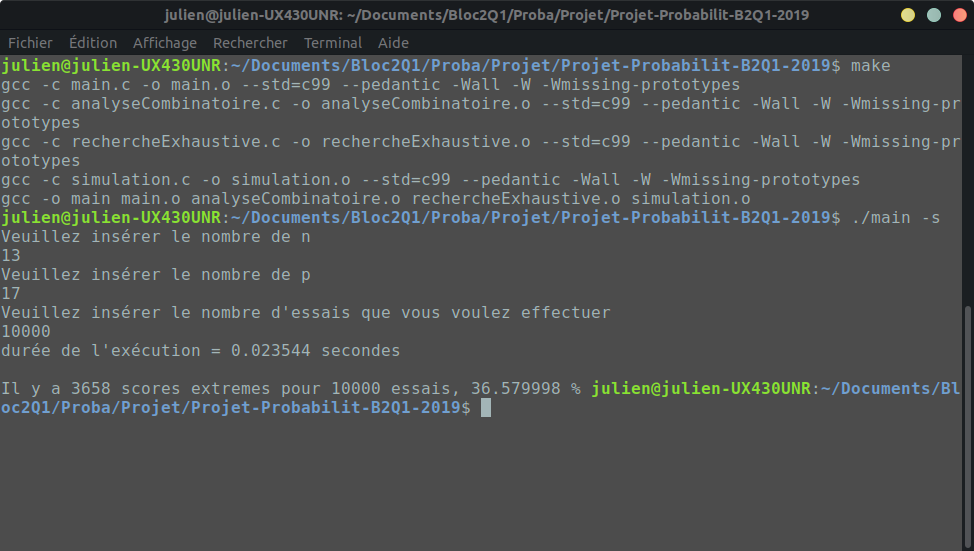
\includegraphics[scale=0.5]{exemple.png}
			\caption{Exemple}
		\end{figure}

\end{enumerate}

\newpage
\section{Limites du programme}
\subsection{Limites avec une durée infinis
}

\begin{figure}[!h]
			\centering
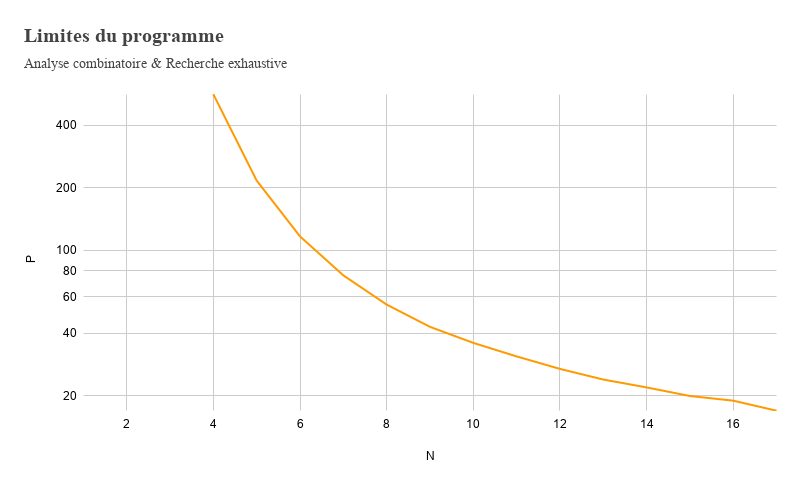
\includegraphics[scale=0.35]{Limites.png}
			\caption{Graphique montrant les limites du programme}
		\end{figure}

\begin{wrapfigure}[22]{l}{4cm}
\includegraphics[scale=0.5]{stats1.png}
\caption{Tableau sur le quel le graphique est basé ( pour un \textit{p} compris entre deux valeurs de ce tableau il est plus judicieux de choisir un \textit{n} borné vers le bas, exemple : \textit{p} = 18 et \textit{n} = 17}
\label{Tableau}
\end{wrapfigure}

Pour un temps infinis le programme qui est compilé en \textbf{analyse combinatoire} ou \textbf{recherche exhaustive} peut gérer aux maximums ces cas ci ( voir tableau ) en effet la plus part des valeurs, dont celle qui stocke le nombres de "n-p mots" sont des \textsc{unsigned int} ainsi le nombre de mots différents possible est : $2^{32}-1$. Pour trouver ces résultats il a juste fallu calculer les \textit{n} et \textit{p} maximum pour les quels $\comb_{n+p}^n$ $\leq 2^{32}-1$.
Bien évidement \textit{n} et \textit{p} sont interchangeable. \\ \\Pour la \textbf{simulation}, c'est un peu différent, la limite réside dans le nombres d'essais et doit donc être inférieur ou égale à $2^{32}-1$. \\ \\ Cependant en pratique le programme n'est pas tellement efficace pour des nombres aussi élevé... Prenons un \textit{n} égale à 13 et un \textit{p} égale à 24 par exemple, l’exécution du programme prends $\sim$ 143 secondes... Ce qui est énorme et donc pas tellement utilisable. Dans ce genre de situation la simulation bien que moins "correcte" sera plus intéressante, en effet pour un \textit{n} et \textit{p} équivalent et un nombres d'essais élevé nous tombons sur une réponses presque équivalente en moins de 6 secondes. 
\\
     \begin{figure}[!h]
			\centering
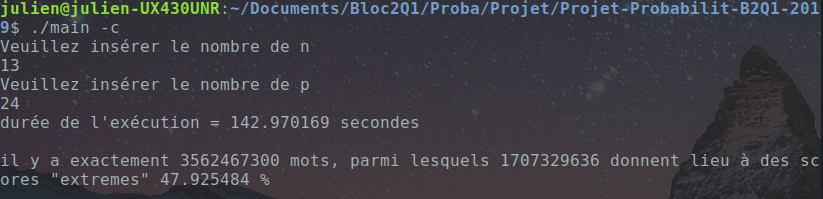
\includegraphics[scale=0.25]{exemple2.png}
			\caption{Exemple d’exécution}
		\end{figure}


\newpage

\subsection{Limites avec une durée finie ( 15 secondes )}
Le graphique ci-dessous montres les \textit{n} et \textit{p} maximum pour les quels la compilation prends moins de quinze secondes, ce qui rend ainsi le programme beaucoup plus utilisable.
\begin{figure}[!h]
			\centering
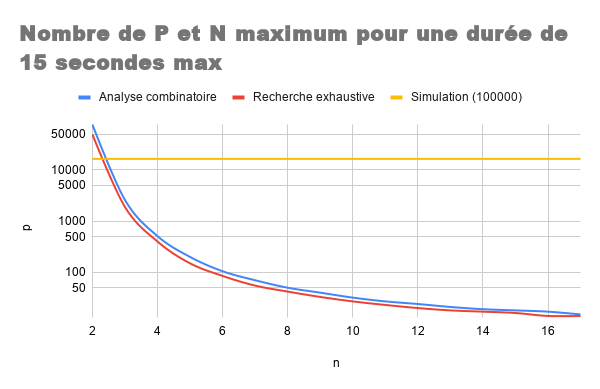
\includegraphics[scale=0.4]{graphique2.png}
		\end{figure}

Nous pouvons constater des phénomènes intéressant, déjà l'analyse combinatoire et la recherche exhaustive sont assez proche, bien que l'analyse combinatoire reste la plus efficace des deux, nous pouvons utiliser des nombres plus élevé pour un résultat plus rapide. Cependant la simulation (1000000 essais) qu’importe le nombre de \textit{n}  ou \textit{p} $\leq 16500$. La compilation prendra moins de quinze secondes et restera à ce temps fixe, ce qui peut être fortement utile si nous recherchons des approximations.
\begin{figure}[!h]
\centering
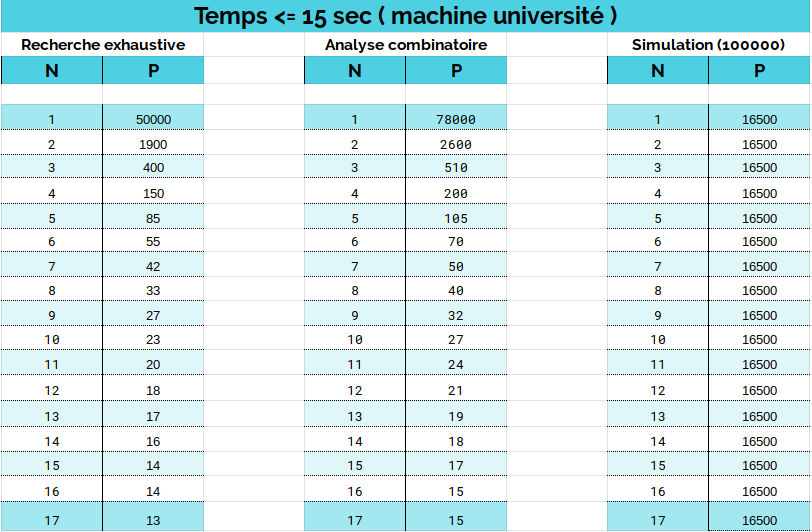
\includegraphics[scale=0.5]{tableau2.png}
\caption{Tableau sur le quel le graphique est basé}

Tous ces tests ont été fait sur les machines de l'université et montre ainsi les limites du programme.
\end{figure}
\newpage



\end{document}
